Ziel dieses Versuchs ist es, die mechanischen Eigenschaften von Kupfer-Scherkörpern zu
untersuchen und zu vergleichen:\\
\subsection{Untersuchung der Prüfkörper:}
Hiermit werden zwei Kupfer-Scherkörpern untersucht mit jeweils eine Art:\\
Scherprüfling 1: Versilberter Kupfer Scherkörper gesintert auf Kupferbodenplatte.\\
\vspace{0.05cm}
\begin{figure}[h]
    \centering
    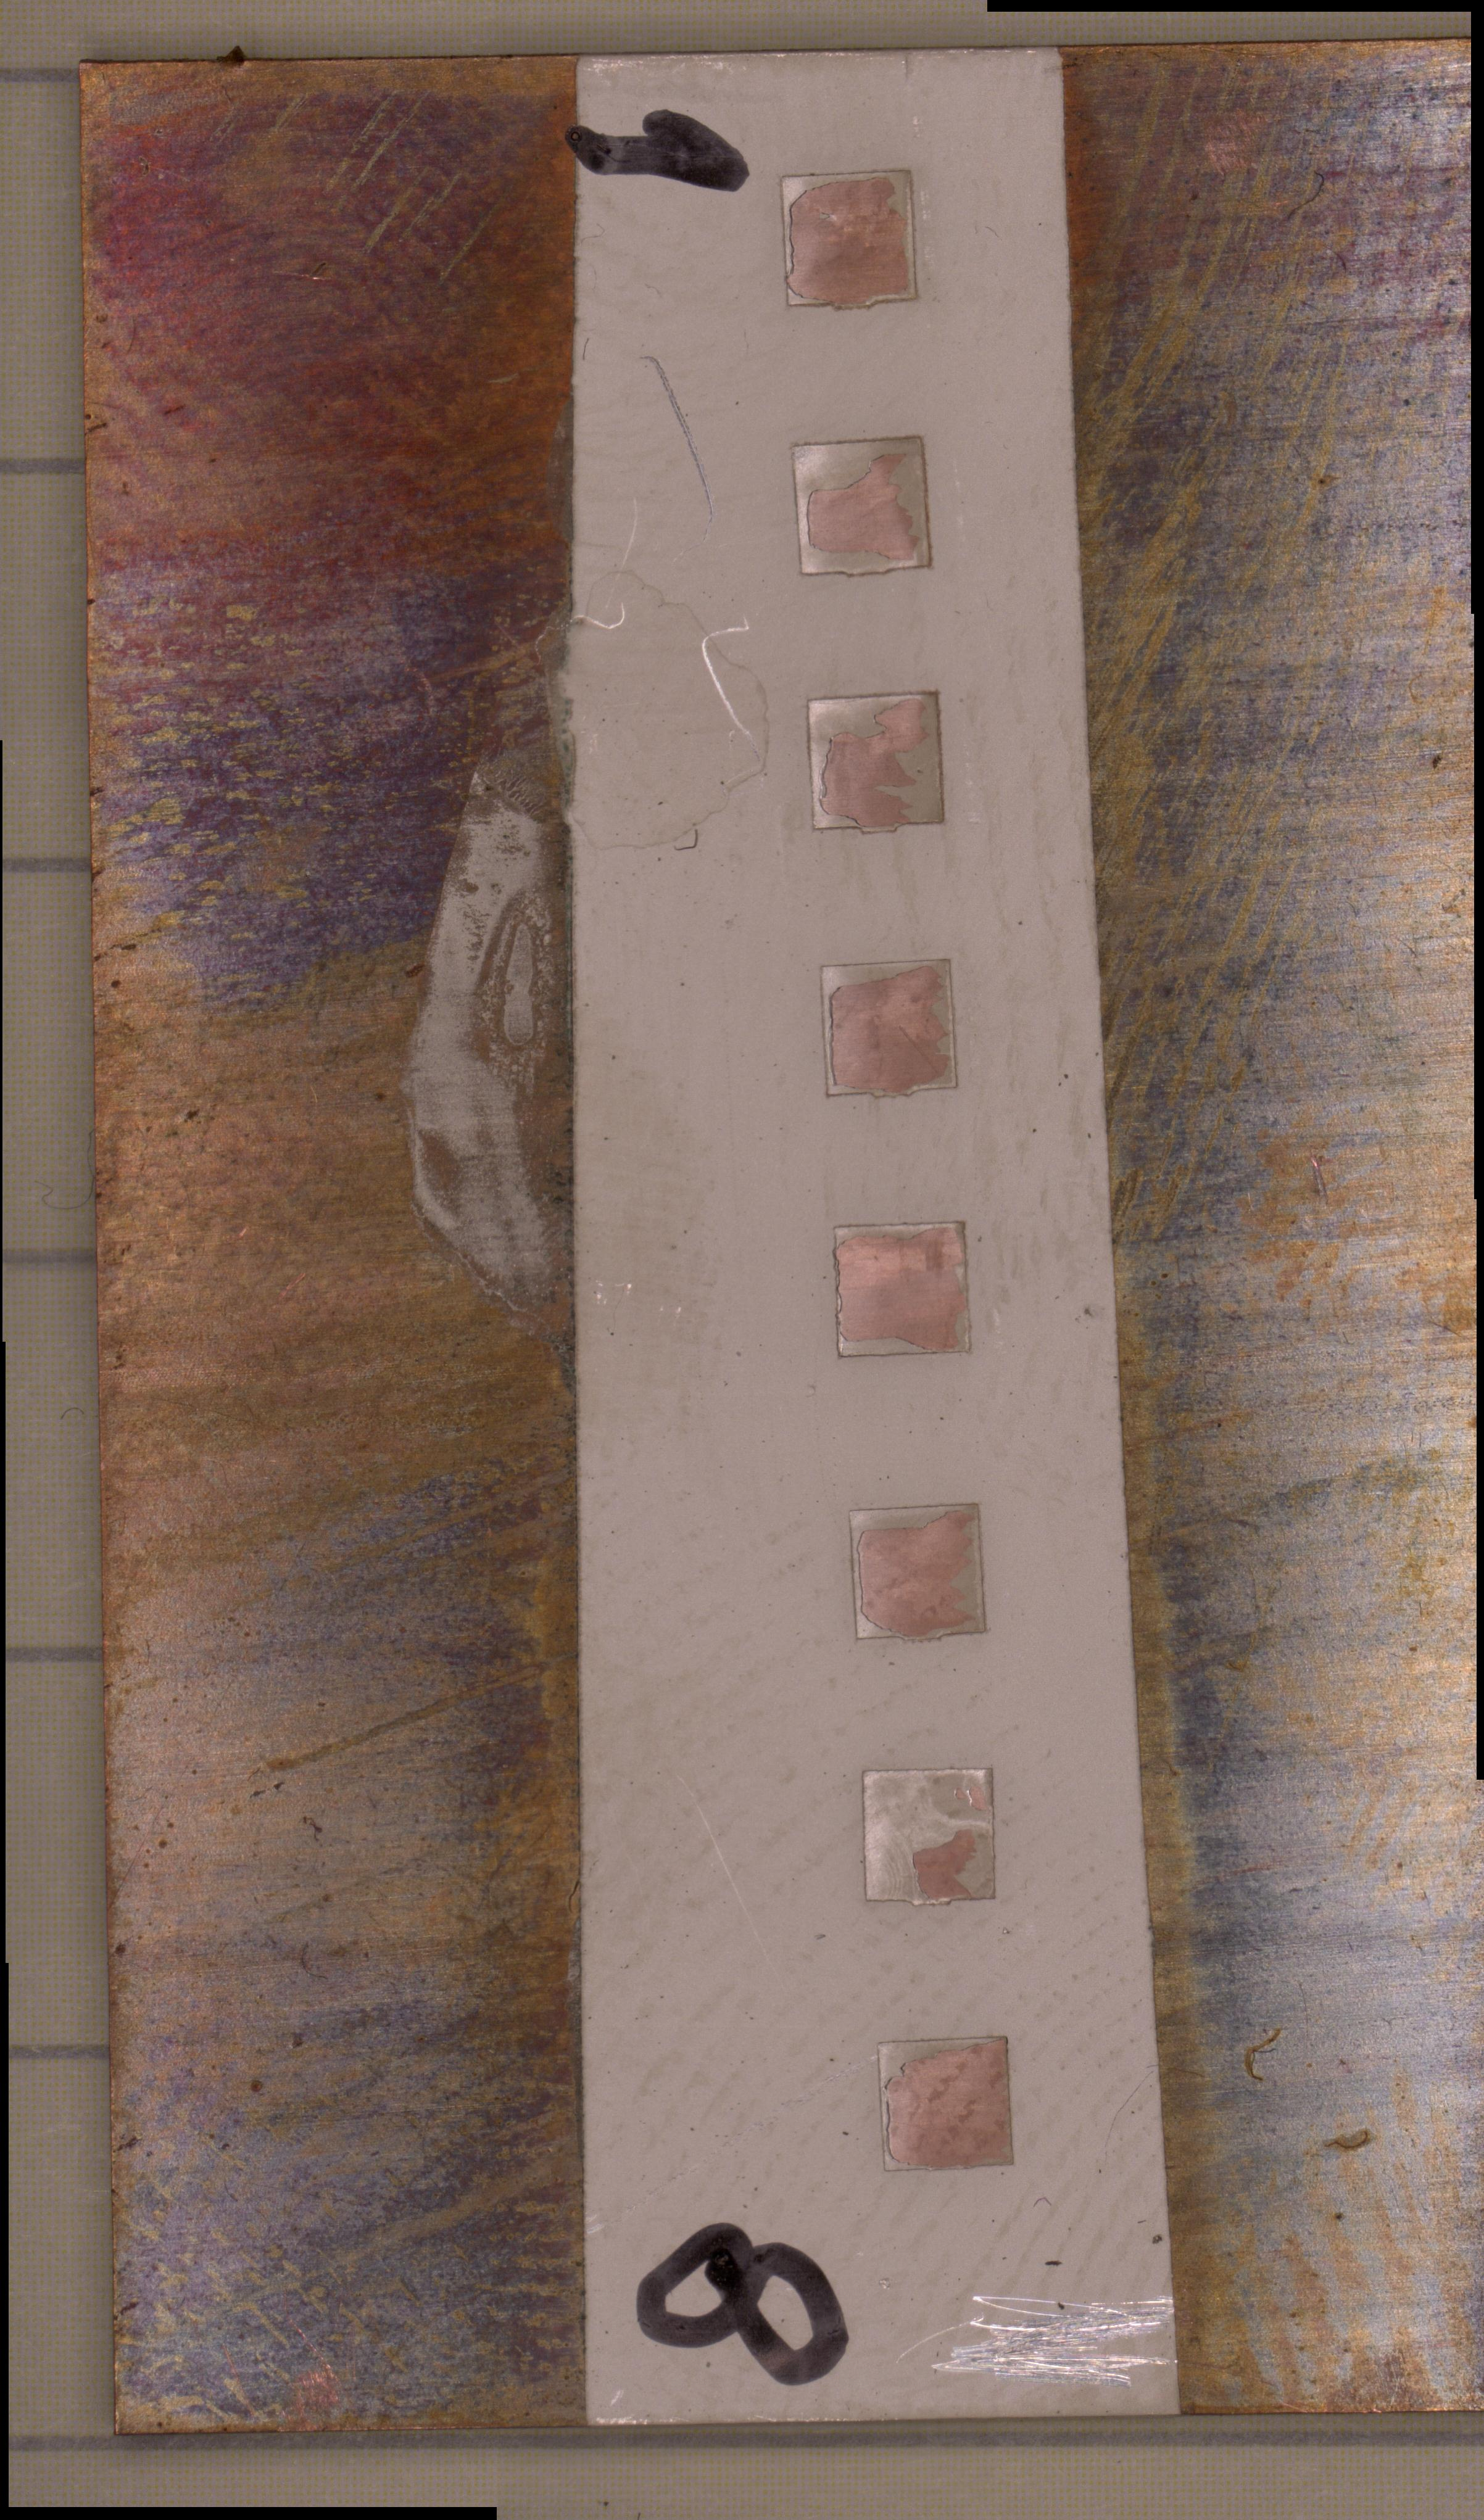
\includegraphics[scale=0.1, angle=90]{Bilder/Bodenplatte_Sintern_Gesamt.jpg}
    \caption{Scherprüfling gesintert}
    \vspace{0.2cm}
    \label{Abb.2: Scherprüfling gesintert}
\end{figure}\\
Scherprüfling 2: Kupfer Scherkörper laminiert auf Kupferbodenplatte
\vspace{0.1cm}
\begin{figure}[h]
    \centering
    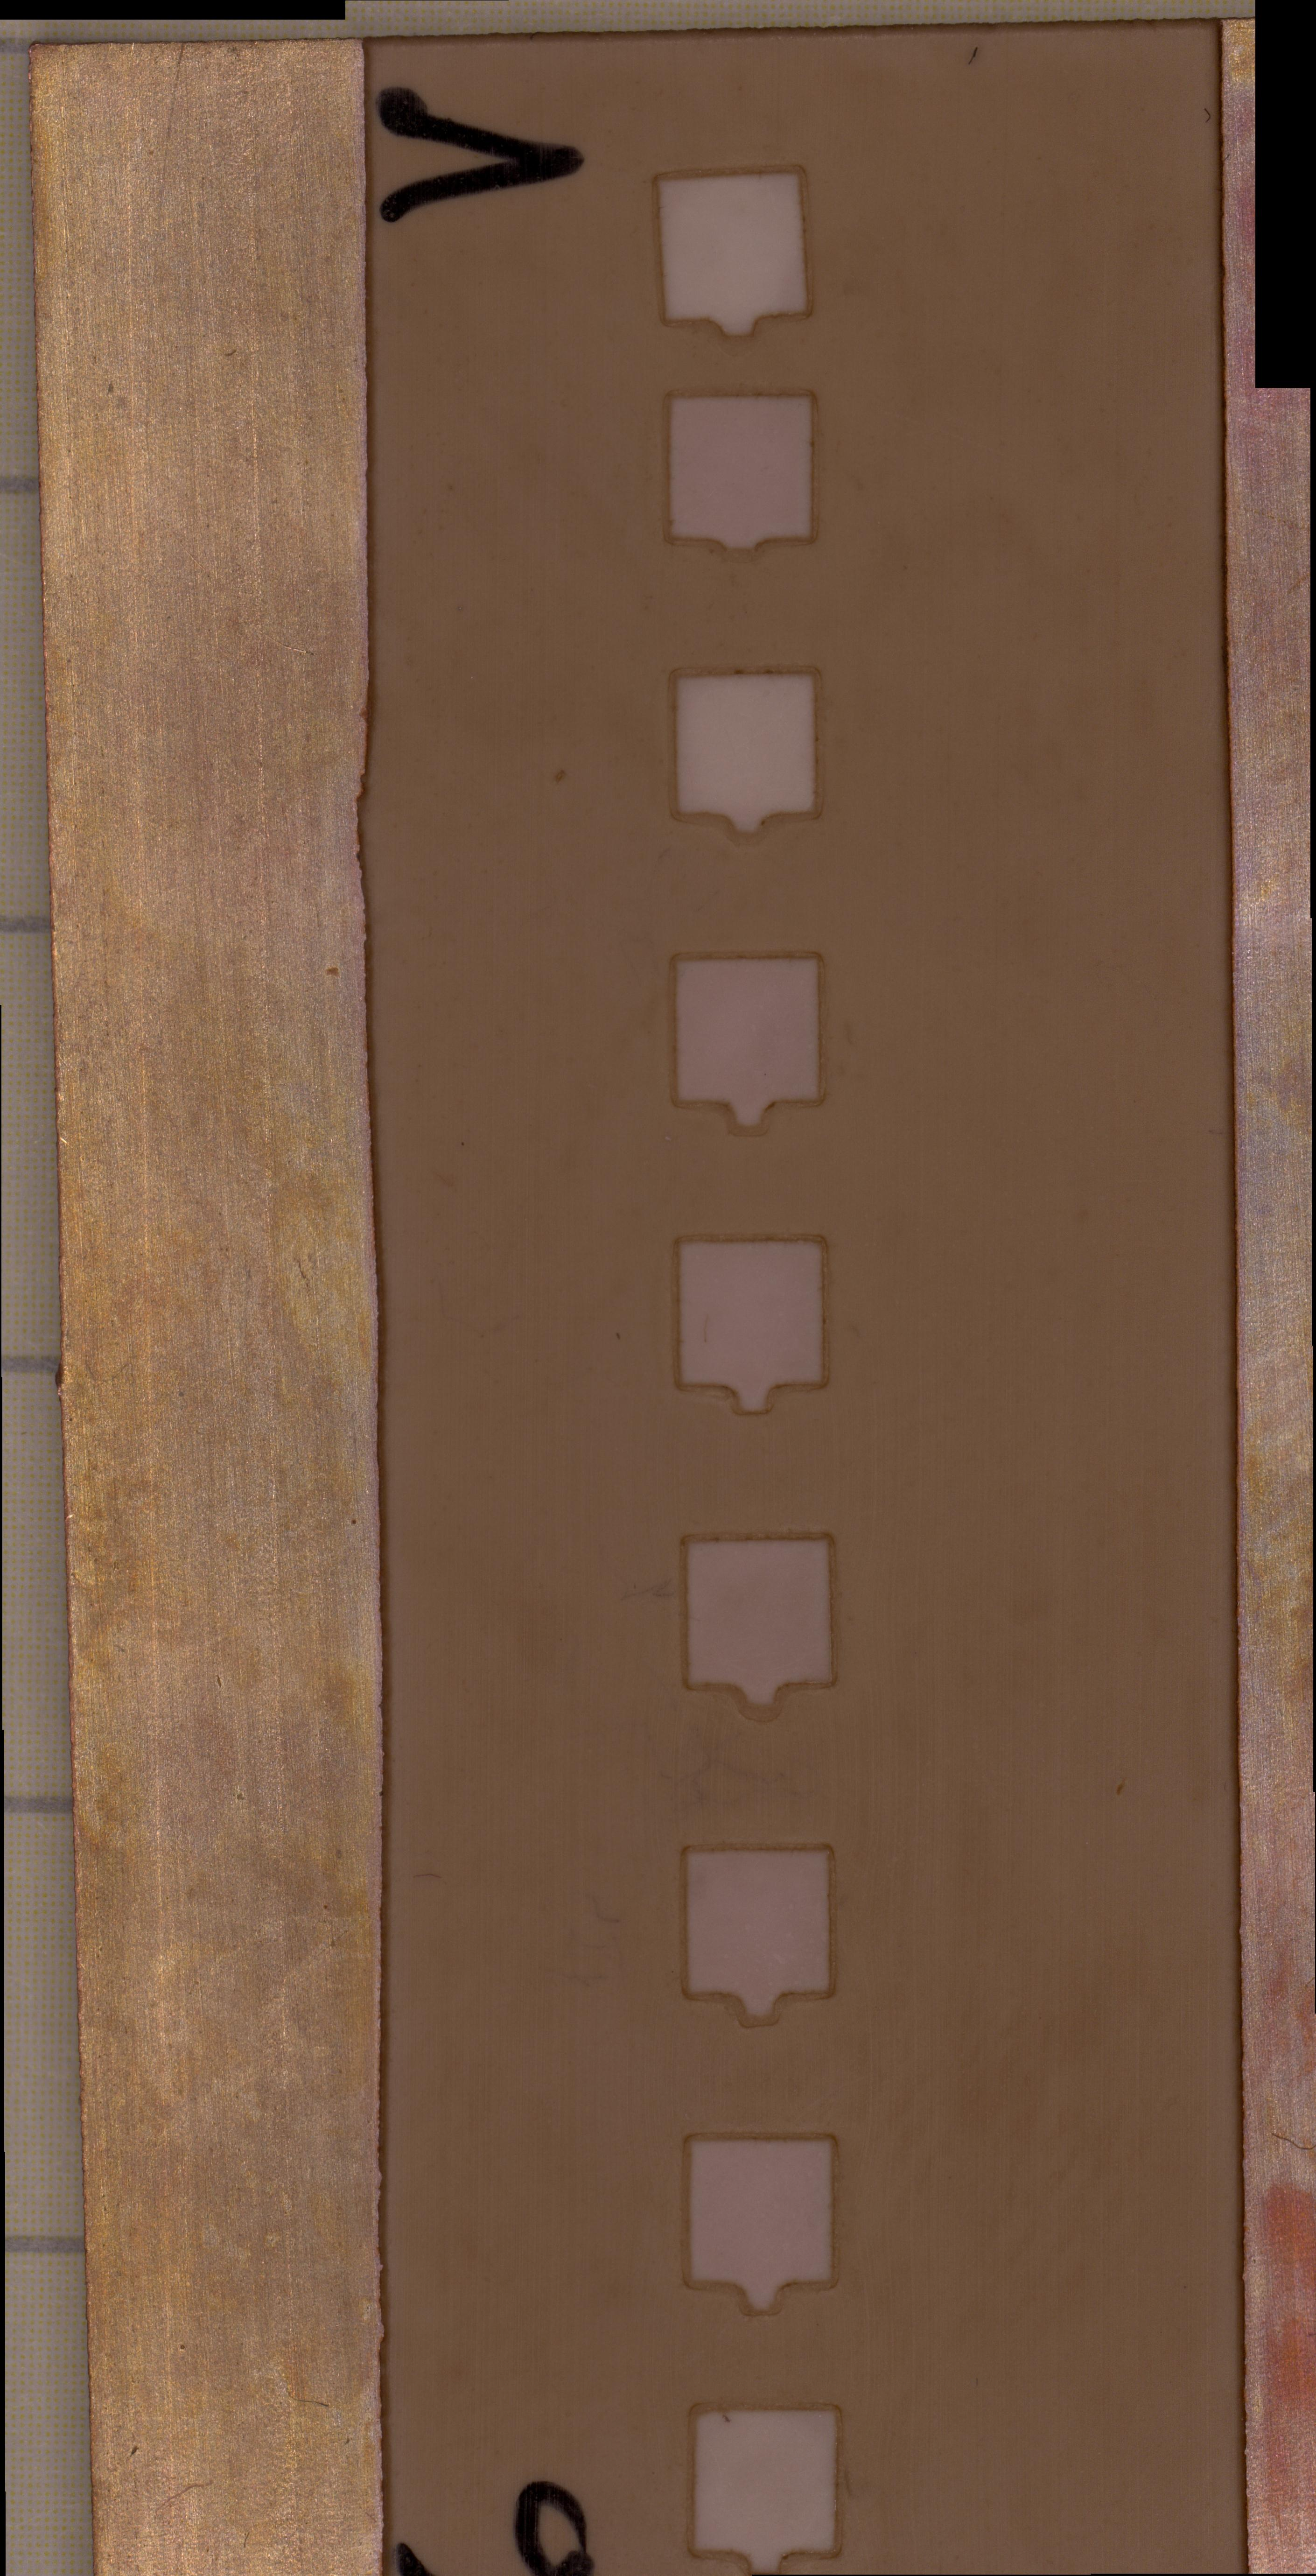
\includegraphics[scale=0.075, angle=90]{Bilder/Laminieren_Bodenplatte_Gesamt.jpg}
    \caption{Scherprüfling laminiert}
    \vspace{0.2cm}
    \label{Abb.3: Scherprüfling laminiert}
\end{figure}
\subsection{Durchführung:}
Jeder Prüfling besitzt in seiner Platte zehn Scherkörper, die durch Schubspannung mit einem Schermeißel abgeschert werden.
\vspace{0.1cm}
\begin{figure}[h]
    \centering
    \includegraphics[scale=0.4]{Bilder/Schermeißel.png}
    \caption{Scherablauf}
    \vspace{0.2cm}
    \label{Abb.4: Scherablauf}
\end{figure}
\vspace{0.1cm}
Jeder der Prüfkörper wird nach dem Scheren auf eine Karteikarte geklebt, wobei der jeweilige Kraftwert eingetragen wird.
Dieser Wert wird aus der Computersoftware abgelesen.
\subsection{Untersuchung}
Nach Durchführung der Scherversuche werden die Bruchstellen der Prüfkörper mithilfe eines Digitalmikroskops untersucht und festgehalten.
Dabei steht die Identifizierung und Analyse der entstandenen Bruchmuster im Fokus.